\documentclass[10pt]{beamer}

\input{/Users/daniel/Documents/LaTeX/beamer-style.tex}

\title{SGBD - 2\textsuperscript{e}}
\subtitle{PL-SQL - Chapitre 6 - Des records aux collections bulk}
\date{\today}
\author{Daniel Schreurs}
\institute{Haute École de Province de Liège}
%\titlegraphic{\hfill\includegraphics[height=1.5cm]{logo.eps}}

\begin{document}
\maketitle

\setbeamerfont{subsection in toc}{size=\small}
\setbeamerfont{subsubsection in toc}{size=\normalsize}
\setbeamertemplate{section in toc}[sections numbered]
\setbeamertemplate{subsection in toc}[subsections numbered]
\setbeamertemplate{subsubsection in toc}[subsubsections numbered]
\begin{frame}[allowframebreaks]{Table des matières du chapitre}
    \tableofcontents[subsectionstyle=show/show/hide,subsubsectionstyle=show/show/hide,]
\end{frame}

\section{Introduction}
\tocss
\subsection{Définitions}
\begin{frame}{\secname : \subsecname}
    \metroset{block=fill}
    \begin{alertblock}{Important}
        Les records\footnote{Coir structures en langage C} permettent de définir des structures de données hétérogènes.
    \end{alertblock}
\end{frame}
\subsection{Exemple 1}

\begin{frame}{\secname : \subsecname}
    \lstinputlisting[language=plsql, title=Exemple 1]{../exemples/PLSQL Chapitre 6/exemple1.sql}
\end{frame}

\begin{frame}{\secname : \subsecname}
    \lstinputlisting[language=plsql, title=Exemple 1 - avec \%type ]{../exemples/PLSQL Chapitre 6/exemple1-1.sql}
\end{frame}



\begin{frame}{\secname : \subsecname}
    \lstinputlisting[language=plsql, title=Exemple 1 - avec \%ROWTYPE]{../exemples/PLSQL Chapitre 6/exemple1-2.sql}
\end{frame}

\begin{frame}[standout]
    Peut-on se passer des types record ?
\end{frame}
\section{Opérateurs}
\tocss
\subsection{Opérateur d’accession}
\begin{frame}{\secname : \subsecname}
    \lstinputlisting[language=plsql, title=Exemple 2]{../exemples/PLSQL Chapitre 6/exemple2.sql}
\end{frame}
\subsection{Comparaison}
\begin{frame}{\secname : \subsecname}
    \metroset{block=fill}
    \begin{alertblock}{Important}
        Pour \textbf{comparer deux records}, il faut les comparer champ par champ.
        L'idéal est donc d'écrire une fonction qui prend 2 records en paramètres et renvoie vrai ou faux
    \end{alertblock}
\end{frame}

\begin{frame}{\secname : \subsecname}
    \lstinputlisting[language=plsql, title=Comparaison erronée]{../exemples/PLSQL Chapitre 6/exemple3.sql}
\end{frame}

\begin{frame}{\secname : \subsecname}
    \lstinputlisting[language=plsql, title=Comparaison dangereuse]{../exemples/PLSQL Chapitre 6/exemple3-2.sql}
\end{frame}

\begin{frame}{\secname : \subsecname}
    \lstinputlisting[language=plsql, title=Comparaison OK]{../exemples/PLSQL Chapitre 6/exemple3-3.sql}
\end{frame}

\subsection{Affectation multiple}

\begin{frame}{\secname : \subsecname}
    \lstinputlisting[language=plsql, title=INSERT INTO]{../exemples/PLSQL Chapitre 6/exemple4.sql}
\end{frame}

\begin{frame}{\secname : \subsecname}
    \lstinputlisting[language=plsql, title=UPDATE Dept SET]{../exemples/PLSQL Chapitre 6/exemple5.sql}
\end{frame}

\subsection{RETURNING INTO}
\begin{frame}{\secname : \subsecname}
    \metroset{block=fill}
    \begin{alertblock}{Important}
        L'utilisation de la clause \lstinline[language=plsql]!RETURNING INTO! dans les commandes \lstinline[language=plsql]!insert!, \lstinline[language=plsql]!update! et \lstinline[language=plsql]!delete! évite de refaire une nouvelle lecture pour connaitre les nouvelles (ou anciennes) valeurs d'une ligne!
    \end{alertblock}
    \centerline{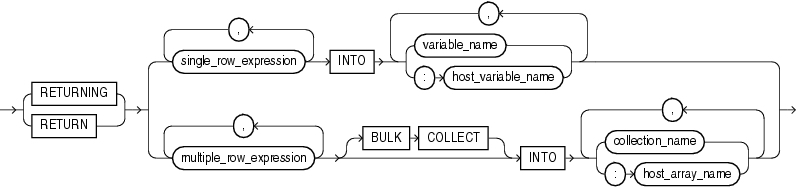
\includegraphics[width=\textwidth]{../assets/img/returning_clause.jpg}}
\end{frame}


\begin{frame}{\secname : \subsecname}
    \lstinputlisting[language=plsql, title=UPDATE Dept SET]{../exemples/PLSQL Chapitre 6/exemple6.sql}
\end{frame}


\begin{frame}{\secname : \subsecname}
    \lstinputlisting[language=plsql, title=Rappel ! Recherche d'UN tuple]{../exemples/PLSQL Chapitre 6/exemple7.sql}\footnote{Attention, si critère de recherche ne porte pas sur la clé primaire, prévoir également le \lstinline[language=plsql]!TOO_MANY_ROWS! !!!}
\end{frame}

\subsection{BULK COLLECT INTO}
\begin{frame}{\secname : \subsecname}
    \lstinputlisting[language=plsql, title=Recherche de PLUSIEURS tuples]{../exemples/PLSQL Chapitre 6/exemple8.sql}
\end{frame}

\begin{frame}{\secname : \subsecname}
    \metroset{block=fill}
    \begin{alertblock}{Important}
        Avec \lstinline[language=plsql]!BULK COLLECT INTO!, \lstinline[language=plsql]!NO_DATA_FOUND! n'est pas déclenchée lorsque le résultat de la recherche est vide !
    \end{alertblock}
\end{frame}

\subsection{FORALL}
\begin{frame}{\secname : \subsecname}
    \begin{itemize}
        \item L'instruction \lstinline[language=plsql]!FORALL! permet d'envoyer en une fois un lot d'instructions SQL et les collections \lstinline[language=plsql]!bulk! permettent de récupérer les résultats;
        \item Pour accélérer le traitement des instructions, \lstinline[language=plsql]!insert!, \lstinline[language=plsql]!update! ou \lstinline[language=plsql]!delete!, on les place dans un \lstinline[language=plsql]!forall! plutôt que dans une boucle classique. Pour optimiser les instructions \lstinline[language=plsql]!select!, on utilise la clause \lstinline[language=plsql]!into bulk collect! !
    \end{itemize}
\end{frame}

\begin{frame}{\secname : \subsecname}
    \lstinputlisting[language=plsql, title=Rappel : la boucle FOR]{../exemples/PLSQL Chapitre 6/exemple9.sql}
\end{frame}

\begin{frame}[allowframebreaks]{\secname : \subsecname}
    \lstinputlisting[language=plsql, title=FORALL i IN]{../exemples/PLSQL Chapitre 6/exemple10.sql}
\end{frame}

\begin{frame}[allowframebreaks]{\secname : \subsecname}
    \lstinputlisting[language=plsql, title=Récupérer les employés supprimés]{../exemples/PLSQL Chapitre 6/exemple11.sql}
\end{frame}


\begin{frame}[allowframebreaks]{\secname : \subsecname}
    \metroset{block=fill}
    \begin{alertblock}{Important}
        Dans une instruction \lstinline[language=plsql]!FORALL!, si l'exécution d'une instruction SQL provoque le déclenchement d'une \textbf{exception} non gérée, toutes les modifications réalisées par \textbf{les instructions précédentes seront annulées}\footnote{Sauf si l'exception est gérée.}.
    \end{alertblock}
\end{frame}

\begin{frame}[allowframebreaks]{\secname : \subsecname}
    \lstinputlisting[language=plsql, title=FORALL et exception gérée]{../exemples/PLSQL Chapitre 6/exemple12.sql}
\end{frame}

\subsection{SQL\%BULK\_ROWCOUNT}
\begin{frame}{\secname : \subsecname}
    Le nombre de lignes impliquées dans chaque instruction LMD d'un FORALL peut être déterminé au moyen de l'attribut composé \lstinline[language=plsql]!SQL\%BULK_ROWCOUNT!.\footnote{Cet attribut est un tableau PL/SQL dont le nième élément contient le nombre de lignes traitées dans la nième instruction LMD contenue dans un FORALL}
\end{frame}

\subsection{save exceptions}
\begin{frame}{\secname : \subsecname}
    \begin{itemize}
        \item PL/SQL possède un mécanisme pour gérer les exceptions déclenchées pendant l'exécution d'un FORALL.
        \item Ce mécanisme, déclenché par la clause \lstinline[language=plsql]!save exceptions!, permet de sauver les informations sur les exceptions et de continuer le traitement des instructions.
        \item L'absence de cette clause dans une instruction FORALL provoque l'arrêt de l'instruction dès la première exception rencontrée.
    \end{itemize}
\end{frame}


\begin{frame}{\secname : \subsecname}
    Avec la clause SAVE EXCEPTIONS, toutes les exceptions détectées pendant l'exécution de FORALL sont sauvées dans l'attribut \lstinline   [language=plsql]!\%BULK_EXCEPTIONS (table PL_SQL)!.
    \begin{itemize}
        \item \lstinline[language=plsql]!SQL\%BULK_EXCEPTIONS.COUNT! : nombre d'exceptions rencontrées pendant l'exécution du FORALL
        \item \lstinline[language=plsql]!SQL\%BULK_EXCEPTIONS(i).ERROR_INDEX! : indice de l'itération qui a provoqué l'exception
        \item \lstinline[language=plsql]!SQL_BULK_EXCEPTIONS(i).ERROR_CODE! : code d'erreur d'Oracle
    \end{itemize}
\end{frame}

\begin{frame}[allowframebreaks]{\secname : \subsecname}
    \lstinputlisting[language=plsql, title=Gestion des exceptions dans FORALL]{../exemples/PLSQL Chapitre 6/exemple13.sql}
\end{frame}

\begin{frame}[allowframebreaks]{\secname : \subsecname}
    \lstinputlisting[language=plsql, title=RETURNING...BULK COLLECT INTO]{../exemples/PLSQL Chapitre 6/exemple13.sql}
\end{frame}

\section{Résumé}
\tocss
\subsection{Recherche d'un seul tuple}
\begin{frame}{\secname : \subsecname}
    \lstinline[language=plsql]!SELECT ... INTO ... FROM ... WHERE ... ;!
    \begin{itemize}
        \item Le tuple est trouve : l'exécution continue
        \item Le tuple n'est pas trouvé :
              exception \lstinline[language=plsql]!NO_DATA_FOUND!
        \item La sélection renvoie plus d'un tuple
              exception \lstinline[language=plsql]!TOO_MANY_ROWS!
    \end{itemize}
\end{frame}

\begin{frame}{\secname : \subsecname}
    \lstinputlisting[language=plsql, title=La boucle FOR]{../exemples/PLSQL Chapitre 6/exemple15.sql}
    \begin{itemize}
        \item Un ou plusieurs tuples sélectionnés => exécution LOOP
        \item Aucun tuple sélectionné => pas exécution LOOP, on continue l'exécution après LOOP
        \item PAS d'exception \lstinline[language=plsql]!NO_DATA_FOUND! déclenchée !!!
    \end{itemize}
\end{frame}

\subsection{Recherche de plus d'un tuple, initialisation d'une collection de records}
\begin{frame}{\secname : \subsecname}
    \lstinputlisting[language=plsql, title=BULK COLLECT INTO]{../exemples/PLSQL Chapitre 6/exemple16.sql}
    \begin{itemize}
        \item Un ou plusieurs tuples sélectionnés => initialisation de la VariableTable indicée de 1 à n
        \item Aucun tuple sélectionné => on continue l'exécution après le \lstinline[language=plsql]!SELECT!
        \item PAS d'exception \lstinline[language=plsql]!NO_DATA_FOUND! déclenchée !!!
    \end{itemize}
\end{frame}

\subsection{BULK\_EXCEPTIONS}
\begin{frame}{\secname : \subsecname}
    \begin{itemize}
        \item Option \lstinline[language=plsql]!SAVE EXCEPTIONS! permet de sauver toutes les exceptions détectées pendant l’exécution de \lstinline[language=plsql]!FORALL! dans une table PL/SQL et de continuer le traitement.
        \item \lstinline[language=plsql]!SQL\%BULK_EXCEPTIONS.COUNT! le nombre d’exceptions rencontrées pendant l’exécution du \lstinline[language=plsql]!FORALL!
        \item \lstinline[language=plsql]!SQL\%BULK_EXCEPTIONS(i).ERROR_INDEX! contient l’indice de l’itération qui a provoqué l’exception
        \item \lstinline[language=plsql]!SQL\%BULK_EXCEPTIONS(i).ERROR_CODE! contient le code d’erreur d’Oracle
        \item Le nième élément de \lstinline[language=plsql]!SQL\%BULK_ROWCOUNT! contient le nombre de lignes traitées dans la nième instruction LMD
    \end{itemize}
\end{frame}



\end{document}
